\documentclass[11pt,a4paper]{article}

\usepackage[T1]{fontenc}
\usepackage[utf8]{inputenc}
\usepackage[margin=1.05in]{geometry}
\usepackage{amsmath,amssymb,amsthm,mathtools}
\usepackage{booktabs}
\usepackage{graphicx}
\usepackage[protrusion=true,expansion=false]{microtype}
\usepackage{siunitx}
\usepackage{caption}
\usepackage{enumitem}
\usepackage[table]{xcolor}
\usepackage[hidelinks,breaklinks]{hyperref}
\usepackage{cleveref}

\sisetup{detect-weight=true, group-separator={,}}

% --- theorem environments -------------------------------------------------
\theoremstyle{definition}
\newtheorem{definition}{Definition}[section]
\theoremstyle{plain}
\newtheorem{proposition}[definition]{Proposition}
\newtheorem{theorem}[definition]{Theorem}
\newtheorem{lemma}[definition]{Lemma}
\newtheorem{corollary}[definition]{Corollary}
\theoremstyle{remark}
\newtheorem{remark}[definition]{Remark}
\newtheorem{assumption}[definition]{Assumption}

% --- notation -------------------------------------------------------------
\newcommand{\R}{\mathbb{R}}
\newcommand{\E}{\mathbb{E}}
\newcommand{\Prob}{\mathbb{P}}
\newcommand{\Var}{\operatorname{Var}}
\newcommand{\Cov}{\operatorname{Cov}}
\newcommand{\Corr}{\operatorname{Corr}}
\newcommand{\CV}{\operatorname{CV}}
\newcommand{\simplex}{\Delta}
\newcommand{\one}{\mathbf{1}}
\newcommand{\VOLL}{\mathrm{VOLL}}
\newcommand{\MW}{\,\mathrm{MW}}
\DeclareMathOperator*{\argmax}{arg\,max}
\DeclareMathOperator*{\argmin}{arg\,min}

% Hawaiian okina (glottal stop); ASCII-safe approximation
\newcommand{\okina}{\textquoteleft}

\captionsetup{font=small,labelfont=bf}

\title{\bfseries Radial and Angular Risk in Stochastic\\ DC Optimal Power Flow:\\[0.25em]
\large How Distributional Misspecification Relocates,\\ Rather Than Merely Inflates, Estimated Grid Risk}

\author{Pascual Z\'arate\thanks{The University of Chicago, Class of 2029.
Prepared as Problem Set 8 of an ongoing research project on island power-system
optimisation. Code, data and all numerical results are reproducible from the
repository described in \Cref{app:repro}.}}

\date{8 September 2026}

\begin{document}
\maketitle

\begin{abstract}
\noindent
We study a Monte Carlo adequacy experiment in which a fixed transmission network
is solved under $N = \num{10000}$ independent realisations of nodal demand. The
dispatch model is a DC optimal power flow augmented with load shedding priced at
the value of lost load, which renders the program feasible for every demand
realisation and converts ``infeasibility'' from a Boolean solver outcome into a
measurable quantity in megawatts. We establish four structural results. First,
the recourse formulation has relatively complete recourse, and shedding is
optimal only when the zero-shed program is infeasible, provided the value of
lost load exceeds the largest nodal dual---a condition strictly stronger than
exceeding the costliest generator, because congestion rents can drive locational
prices above every unit's marginal cost. Second, under independent exponential
sampling $D_i = \mu_i E_i$ the \emph{system-level} coefficient of variation is
$\sqrt{\sum_i \mu_i^2}\,/\sum_i \mu_i$, which lies in $[n^{-1/2}, 1]$ and is
governed entirely by load concentration. Third, the servable set along any
demand ray is an interval $[0, T^\star(s)]$, so adequacy failure is exactly the
event $\lVert D\rVert_1 > T^\star(D/\lVert D\rVert_1)$: adequacy is an
\emph{angular} quantity. Fourth---and contrary to our initial conjecture---line
congestion is very nearly \emph{radial}: on a $9$-bus model of the O\okina ahu
system a single magnitude threshold $t_c = \SI{585}{\mega\watt}$ reproduces the
congestion frequency under two radically different demand distributions to
within $\SI{0.6}{\percent}$. We then show empirically that replacing the assumed
$\mathrm{Exp}(1)$ marginals with \num{8760} hours of filed utility load data
drives estimated shedding probability from $\SI{19.77}{\percent}$ to exactly
zero while \emph{raising} estimated congestion frequency from
$\SI{58.40}{\percent}$ to $\SI{92.51}{\percent}$. Misspecification therefore does
not simply inflate risk; it moves risk from one failure mode to another. Finally
we note that nameplate capacity overstates deliverable capacity by
$\SI{28.3}{\percent}$ on this network, reducing the apparent
$\SI{43}{\percent}$ reserve margin against the observed annual peak to
$\SI{2.63}{\percent}$.

\medskip
\noindent\textbf{Keywords:} DC optimal power flow; stochastic programming;
relatively complete recourse; resource adequacy; model misspecification;
Monte Carlo simulation.
\end{abstract}

\tableofcontents

% ==========================================================================
\section{Introduction}
% ==========================================================================

A deterministic optimal power flow answers one question: given this network and
this demand, what is the cheapest feasible dispatch? A great deal of practical
interest, however, attaches to a different question---given this network and a
\emph{distribution} over demand, how often does something go wrong, and what
exactly goes wrong. Answering the second question requires re-solving the first
many times, and the answer one obtains is a functional of the assumed demand
distribution as much as of the network.

This paper examines that dependence in a setting where the ``true'' distribution
is available. We fix two networks---the IEEE 14-bus test system and a nine-bus
model of the O\okina ahu (Hawai\okina i) transmission system assembled from
utility filings---and solve each under $N = \num{10000}$ demand realisations. We
ask the three questions a planner would ask:

\begin{enumerate}[label=(Q\arabic*),leftmargin=*]
\item How often is the most expensive generator dispatched?
\item How often is the problem infeasible, i.e.\ how often must load be shed?
\item How often do network elements reach their thermal limits?
\end{enumerate}

The demand model specified at the outset is the natural first choice in the
absence of data: at each load node $i$, draw $D_i = \mu_i E_i$ with
$E_i \sim \mathrm{Exp}(1)$ independent across nodes, so that $\E[D_i] = \mu_i$.
For the O\okina ahu system, however, we possess \num{8760} hours of filed hourly
load. This permits a direct comparison between the answers the assumed
distribution produces and the answers the empirical distribution produces, on a
network that never changes.

\paragraph{Contributions.}
Our contributions are of two kinds. On the structural side
(\Cref{sec:model,sec:demand,sec:geometry}) we characterise the feasible set of
the recourse program and the geometry of its two failure modes. The central
structural observation is a decomposition of failure into a radial component
(the magnitude $\lVert D\rVert_1$) and an angular component (the direction
$D/\lVert D\rVert_1$), and the finding that the two failure modes load onto these
components very differently. On the empirical side
(\Cref{sec:results14,sec:resultsoahu,sec:misspec}) we quantify the misspecification
effect and show that its sign is not constant across failure modes.

\paragraph{A note on how these results were obtained.}
\Cref{prop:congestion-radial} contradicts the conjecture with which this
investigation began. We had expected congestion to be the directional quantity,
on the intuitive grounds that a line binds when power must cross it, and whether
power must cross it depends on \emph{where} demand sits. The conditional
experiment of \Cref{sec:geometry} refutes this cleanly, and the corrected
statement---that adequacy is angular and congestion is radial---is both simpler
and better supported. We record the failed conjecture because the diagnostic
that settled it (conditioning on total demand and comparing failure rates across
demand models) is reusable.

% ==========================================================================
\section{The dispatch model with recourse}\label{sec:model}
% ==========================================================================

\subsection{Network primitives}

\begin{definition}[Network]\label{def:network}
A \emph{network} is a tuple
$\mathcal{N} = (\mathcal{B}, \mathcal{L}, \mathcal{G}, b, f, t, \bar F, p^{\max}, c, g, r, \beta)$
where $\mathcal{B} = \{1,\dots,n_b\}$ indexes buses, $\mathcal{L} = \{1,\dots,n_\ell\}$
branches, $\mathcal{G} = \{1,\dots,n_g\}$ generators;
$f,t : \mathcal{L}\to\mathcal{B}$ give each branch its endpoints;
$b_\ell > 0$ is branch susceptance in per unit; $\bar F_\ell > 0$ its thermal
rating in \si{\mega\watt}; $p^{\max}_g > 0$ generator capacity;
$c_g \ge 0$ generator marginal cost in \si{\per\mega\watt\hour};
$g : \mathcal{G}\to\mathcal{B}$ assigns generators to buses;
$r \in \mathcal{B}$ is the reference (slack) bus; and $\beta > 0$ is the power base.
\end{definition}

We work throughout with the standard linearised (``DC'') power-flow
approximation: branch resistance and reactive power are neglected, voltage
magnitudes are held at unity, and branch flow is proportional to the phase-angle
difference across the branch.

\begin{assumption}[Standing assumptions]\label{ass:standing}
$(i)$ The network is connected. $(ii)$ Generator minimum stable output is set to
zero, $p^{\min}_g = 0$ for all $g$. $(iii)$ Generator cost is affine with zero
fixed term, so total cost is $\sum_g c_g P_g$.
\end{assumption}

\Cref{ass:standing}$(ii)$ deserves comment because it is consequential. The
O\okina ahu fleet described in \Cref{sec:data} carries \SI{531}{\mega\watt} of
nameplate minimum stable output. Enforcing those bounds inside a continuous
linear program, without the binary commitment variables that would permit a unit
to be switched off, would render every sufficiently \emph{low} demand
realisation infeasible---for reasons of unit commitment rather than of adequacy.
Since this study concerns whether the system can \emph{meet} demand, we permit
the fleet to shut down freely. \Cref{ass:standing}$(iii)$ discards the quadratic
term present in the IEEE-14 cost data; we return to its consequences in
\Cref{rem:linear-cost}.

\subsection{The recourse program}

\begin{definition}[Recourse dispatch program]\label{def:program}
Given a network $\mathcal{N}$, a demand vector $D \in \R^{n_b}_{\ge 0}$, and a
penalty $\VOLL > 0$, define
\begin{subequations}\label{eq:lp}
\begin{align}
\mathcal{P}(D):\quad
\min_{P,\theta,F,S}\quad & \sum_{g\in\mathcal{G}} c_g P_g \;+\; \VOLL \sum_{i\in\mathcal{B}} S_i
  \label{eq:obj}\\
\text{s.t.}\quad
& 0 \le P_g \le p^{\max}_g, && g \in \mathcal{G}, \label{eq:gen}\\
& \theta_r = 0, \label{eq:slack}\\
& F_\ell = \beta\, b_\ell\,\bigl(\theta_{f(\ell)} - \theta_{t(\ell)}\bigr),
  && \ell \in \mathcal{L}, \label{eq:flow}\\
& \sum_{g : g(g)=i} P_g \;-\; (D_i - S_i)
   \;=\; \sum_{\ell : f(\ell)=i} F_\ell - \sum_{\ell : t(\ell)=i} F_\ell,
  && i \in \mathcal{B}, \label{eq:balance}\\
& -\bar F_\ell \le F_\ell \le \bar F_\ell, && \ell \in \mathcal{L}, \label{eq:thermal}\\
& 0 \le S_i \le D_i, && i \in \mathcal{B}. \label{eq:shed}
\end{align}
\end{subequations}
The variable $S_i$ is \emph{load shedding} at bus $i$: demand the system elects
not to serve. We write $C(D)$ for the optimal value of $\mathcal{P}(D)$ and
denote by $\mathcal{P}_0(D)$ the \emph{zero-shed program} obtained by fixing
$S \equiv 0$ (a pure feasibility problem after dropping the objective).
\end{definition}

\begin{definition}[Servable demand]\label{def:servable}
$D$ is \emph{servable} if $\mathcal{P}_0(D)$ is feasible. Write
$\mathcal{S} \subseteq \R^{n_b}_{\ge 0}$ for the set of servable demand vectors.
\end{definition}

The role of \eqref{eq:shed} is methodological rather than physical, and is worth
stating plainly. A Monte Carlo study that omits shedding must detect adequacy
failure by catching an \texttt{INFEASIBLE} status from the solver. That is a poor
instrument on two counts: it is a single bit, carrying no information about the
magnitude of the shortfall, and solvers return the same status for numerical
difficulties unrelated to the physics. Including $S$ makes the program feasible
always, so that failure is reported as a real number---expected unserved energy,
the quantity reliability studies actually use.

\begin{proposition}[Relatively complete recourse]\label{prop:recourse}
For every $D \in \R^{n_b}_{\ge 0}$, $\mathcal{P}(D)$ is feasible and its optimal
value is finite, with $0 \le C(D) \le \VOLL \sum_i D_i$.
\end{proposition}

\begin{proof}
Take $P = 0$, $\theta = 0$, $F = 0$, $S = D$. Constraints \eqref{eq:gen},
\eqref{eq:slack}, \eqref{eq:thermal} and \eqref{eq:shed} hold trivially;
\eqref{eq:flow} holds since $\theta \equiv 0$; and \eqref{eq:balance} reduces to
$0 - (D_i - D_i) = 0$. Hence the feasible set is nonempty. The objective is
bounded below by $0$ since $c \ge 0$ and $\VOLL > 0$, so a finite optimum exists
by LP duality; evaluating the objective at the exhibited point gives the stated
upper bound.
\end{proof}

\Cref{prop:recourse} is the property known in stochastic programming as
\emph{relatively complete recourse}: the second stage is feasible for every
realisation of the random data. It is what licenses the estimator of
\Cref{sec:mc} to be well-defined without conditioning on solver success.

\subsection{Shedding as a last resort}

\Cref{prop:recourse} guarantees feasibility but not that shedding is used only
when unavoidable. If $\VOLL$ were small, the optimiser would shed load
opportunistically whenever generation happened to be expensive, and the reported
``adequacy failures'' would be economic choices rather than physical ones. The
following gives a sufficient condition.

\begin{proposition}[Shedding occurs only under infeasibility]\label{prop:voll}
Let $D \in \mathcal{S}$, let $C_0(D)$ denote the minimum generation cost among
zero-shed feasible points, and let $\lambda^\circ \in \R^{n_b}$ be an optimal dual
vector for the balance constraints \eqref{eq:balance} of that zero-shed problem.
If
\begin{equation}\label{eq:voll-cond}
\VOLL \;>\; \max_{i\in\mathcal{B}} \lambda^\circ_i ,
\end{equation}
then every optimal solution of $\mathcal{P}(D)$ satisfies $S^\star = 0$.
\end{proposition}

\begin{proof}
For $u \in \R^{n_b}_{\ge 0}$ let $V(u)$ be the minimum of $\sum_g c_g P_g$ subject
to \eqref{eq:gen}--\eqref{eq:thermal} with $D$ replaced by $u$, and $V(u) = +\infty$
if no such point exists. $V$ is the value function of a linear program in its
right-hand side, hence convex on its domain, and $\lambda^\circ$ is a subgradient
of $V$ at $D$; therefore
\begin{equation}\label{eq:subgrad}
V(D - S) \;\ge\; V(D) - \langle \lambda^\circ, S\rangle
\qquad\text{for all admissible } S .
\end{equation}
Let $(P,\theta,F,S)$ be feasible for $\mathcal{P}(D)$ with $S \ne 0$. Its
generation cost is at least $V(D-S)$, so its objective satisfies
\[
\sum_g c_g P_g + \VOLL \sum_i S_i
\;\ge\; V(D-S) + \VOLL \sum_i S_i
\;\overset{\eqref{eq:subgrad}}{\ge}\;
C_0(D) + \sum_i \bigl(\VOLL - \lambda^\circ_i\bigr) S_i
\;>\; C_0(D),
\]
the last inequality strict because $S \ne 0$, $S \ge 0$ and
\eqref{eq:voll-cond} holds. Since the zero-shed point attaining $C_0(D)$ is
feasible for $\mathcal{P}(D)$ with objective exactly $C_0(D)$, no solution with
$S \ne 0$ can be optimal.
\end{proof}

\begin{remark}[Why exceeding the costliest generator is not enough]\label{rem:voll}
It is tempting to impose the simpler condition $\VOLL > \max_g c_g$. This is
\emph{insufficient}. The dual $\lambda^\circ_i$ is the locational marginal price
at bus $i$, and in a congested network congestion rent can push it above every
generator's marginal cost; in a companion multi-period study on the same data we
observe locational prices reaching \SI{381}{\per\mega\watt\hour} against a
costliest unit at \SI{237.97}{\per\mega\watt\hour}. In the limit where a bus is
electrically isolated by binding thermal limits, $\lambda^\circ_i$ is unbounded
and no finite $\VOLL$ suffices. We therefore set
$\VOLL = \SI{10000}{\per\mega\watt\hour}$---roughly $42\times$ the costliest
unit---and verify \eqref{eq:voll-cond} \emph{ex post}: across \num{6000} sampled
realisations on the two networks, in every case where the recourse solution shed
load, an independent feasibility test confirmed that $\mathcal{P}_0(D)$ was
genuinely infeasible. There were no counterexamples.
\end{remark}

% ==========================================================================
\section{Demand models}\label{sec:demand}
% ==========================================================================

Throughout, $\mathcal{B}^+ = \{i : \mu_i > 0\}$ denotes the load buses,
$n = |\mathcal{B}^+|$, and $M = \sum_{i} \mu_i$ the design mean total demand.

\subsection{Independent exponential sampling}

\begin{definition}[Model A]\label{def:modelA}
$D_i = \mu_i E_i$ for $i\in\mathcal{B}^+$ and $D_i = 0$ otherwise, where
$E_i \overset{\text{iid}}{\sim} \mathrm{Exp}(1)$.
\end{definition}

Each node then has $\E[D_i] = \mu_i$ and $\operatorname{sd}(D_i) = \mu_i$, so the
\emph{nodal} coefficient of variation is exactly $1$. The system-level dispersion
is quite different, and is determined entirely by how concentrated the load is.

\begin{proposition}[System coefficient of variation]\label{prop:cv}
Under Model A, let $T = \sum_i D_i$. Then $\E[T] = M$,
$\Var(T) = \sum_i \mu_i^2$, and
\begin{equation}\label{eq:cv}
\CV(T) \;=\; \frac{\sqrt{\sum_{i} \mu_i^2}}{\sum_i \mu_i}.
\end{equation}
Moreover
\begin{equation}\label{eq:cvbounds}
\frac{1}{\sqrt{n}} \;\le\; \CV(T) \;\le\; 1,
\end{equation}
with the lower bound attained iff all $\mu_i$ are equal, and the upper bound
attained iff exactly one $\mu_i$ is nonzero.
\end{proposition}

\begin{proof}
Linearity gives $\E[T] = \sum_i \mu_i \E[E_i] = M$. Independence and
$\Var(E_i)=1$ give $\Var(T) = \sum_i \mu_i^2 \Var(E_i) = \sum_i \mu_i^2$, whence
\eqref{eq:cv}. For the bounds, write $\mu = (\mu_i)_{i\in\mathcal{B}^+}$ so that
$\CV(T) = \lVert\mu\rVert_2/\lVert\mu\rVert_1$. The Cauchy--Schwarz inequality
$\lVert\mu\rVert_1 = \langle \mu, \one\rangle \le \sqrt{n}\,\lVert\mu\rVert_2$
gives $\CV(T) \ge n^{-1/2}$, with equality iff $\mu \parallel \one$. The upper
bound is $\lVert\mu\rVert_2 \le \lVert\mu\rVert_1$, valid for nonnegative
vectors, with equality iff $\mu$ has a single nonzero entry.
\end{proof}

\Cref{prop:cv} is the reason a demand model with nodal $\CV = 1$ does not produce
a system with $\CV = 1$: independent nodes diversify. How much they diversify is
a property of the network's load geography, not of the distribution. The two
systems studied here sit at different points of \eqref{eq:cvbounds}, and
\Cref{tab:cv} reports both the analytic value and a $\num{200000}$-draw simulation.

\begin{table}[t]
\centering
\caption{System coefficient of variation under Model A: identity
\eqref{eq:cv} against simulation ($\num{200000}$ draws).}
\label{tab:cv}
\begin{tabular}{lccccc}
\toprule
System & $n$ & $n^{-1/2}$ & Analytic \eqref{eq:cv} & Simulated & Upper bound \\
\midrule
IEEE 14-bus     & 11 & 0.3015 & 0.4439 & 0.4446 & 1 \\
O\okina ahu 9-bus & \phantom{0}8 & 0.3536 & 0.5337 & 0.5330 & 1 \\
\bottomrule
\end{tabular}
\end{table}

O\okina ahu's higher value reflects its load concentration: two buses (Honolulu
and Ewa-Central) carry $\SI{72.4}{\percent}$ of the island. Concentrated load
diversifies less.

\subsection{A common-shock mixture}

Independence across nodes is the strongest assumption in Model A and is
physically implausible: one island shares one weather system and one clock. We
therefore consider a mixture that couples the nodes.

\begin{definition}[Model B]\label{def:modelB}
For a mixing weight $w \in [0,1]$,
\[
D_i \;=\; \mu_i \bigl( w E_0 + (1-w) E_i \bigr),
\]
with $E_0, E_1,\dots \overset{\text{iid}}{\sim} \mathrm{Exp}(1)$; $E_0$ is a
single shock shared by all nodes.
\end{definition}

\begin{proposition}[Induced moments]\label{prop:mixture}
Under Model B, for all $i \ne j$ in $\mathcal{B}^+$:
\begin{align}
\E[D_i] &= \mu_i, \label{eq:mixmean}\\
\CV(D_i) &= \sqrt{w^2 + (1-w)^2} \;=:\; \kappa(w), \label{eq:mixcv}\\
\Corr(D_i, D_j) &= \frac{w^2}{w^2 + (1-w)^2} \;=\; \frac{w^2}{\kappa(w)^2}. \label{eq:mixcorr}
\end{align}
Furthermore $\kappa$ is strictly convex on $[0,1]$, symmetric about $w = 1/2$,
and satisfies $\min_w \kappa(w) = \kappa(1/2) = 1/\sqrt{2}$ and
$\kappa(0)=\kappa(1)=1$.
\end{proposition}

\begin{proof}
\eqref{eq:mixmean} follows from $\E[E_0]=\E[E_i]=1$. By independence and
$\Var(E)=1$, $\Var(D_i) = \mu_i^2\bigl(w^2 + (1-w)^2\bigr)$, giving
\eqref{eq:mixcv}. For $i\ne j$ only the common term contributes to the
covariance, $\Cov(D_i,D_j) = \mu_i\mu_j w^2 \Var(E_0) = \mu_i \mu_j w^2$, and
dividing by $\mu_i\mu_j\kappa(w)^2$ gives \eqref{eq:mixcorr}. Finally
$\kappa(w)^2 = 2w^2 - 2w + 1$ is a strictly convex parabola with vertex at
$w=1/2$ and value $1/2$ there, and value $1$ at both endpoints.
\end{proof}

\begin{remark}[The mixing weight is not a correlation]\label{rem:w}
\Cref{prop:mixture} corrects a natural misreading. The parameter $w$ is a mixing
weight, not a correlation coefficient: at $w = 0.7$ the induced pairwise
correlation is $0.845$, not $0.7$. More importantly, moving $w$ away from $0$
changes \emph{two} quantities at once---it raises correlation and, by the
convexity in \Cref{prop:mixture}, \emph{lowers} nodal dispersion from
$\CV = 1$ to $\kappa(0.7) = 0.762$. Model B is therefore a joint sensitivity,
not a clean isolation of correlation. The construction also cannot produce nodal
$\CV$ below $1/\sqrt2 \approx 0.707$ at any $w$, so it cannot approach the
empirical dispersion reported in \Cref{sec:data}. Simulation with
$\num{200000}$ draws matches \eqref{eq:mixcv}--\eqref{eq:mixcorr} to three
decimal places at every $w \in \{0,0.3,0.5,0.7,1\}$.
\end{remark}

\subsection{Empirical resampling}

\begin{definition}[Model C]\label{def:modelC}
Let $h_1,\dots,h_H$ be the recorded hourly system totals ($H = \num{8760}$) and
let $s \in \simplex^{n_b}$ be a fixed allocation vector with $\sum_i s_i = 1$.
Draw $K \sim \mathrm{Unif}\{1,\dots,H\}$ and set $D = h_K\, s$.
\end{definition}

Model C imposes no distributional assumption on the magnitude. It does, however,
impose a strong assumption on the \emph{direction}: $D/\lVert D\rVert_1 = s$
almost surely. \Cref{sec:geometry} shows this is not innocuous, and
\Cref{sec:limits} treats it as a limitation.

% ==========================================================================
\section{The geometry of failure}\label{sec:geometry}
% ==========================================================================

We now decompose a demand vector into magnitude and direction,
\[
T \;=\; \lVert D \rVert_1 \;=\; \sum_i D_i,
\qquad
\sigma \;=\; D / T \;\in\; \simplex^{n_b},
\]
and ask how each of the two failure modes depends on the pair $(T,\sigma)$.

\subsection{Adequacy is angular}

\begin{proposition}[Rays meet the servable set in an interval]\label{prop:ray}
Fix $\sigma \in \simplex^{n_b}$ and define
$T^\star(\sigma) = \sup\{T \ge 0 : T\sigma \in \mathcal{S}\}$. Then
$T^\star(\sigma) < \infty$, the supremum is attained, and
\[
\{T \ge 0 : T\sigma \in \mathcal{S}\} \;=\; [\,0,\; T^\star(\sigma)\,].
\]
\end{proposition}

\begin{proof}
\emph{Finiteness.} Summing \eqref{eq:balance} over $i\in\mathcal{B}$, the flow
terms cancel in pairs, giving $\sum_g P_g = \sum_i D_i = T$. With
\eqref{eq:gen} this forces $T \le \sum_g p^{\max}_g$, so
$T^\star(\sigma) \le \sum_g p^{\max}_g < \infty$.

\emph{Downward closure.} Suppose $T\sigma \in \mathcal{S}$, witnessed by
$(P,\theta,F)$ satisfying \eqref{eq:gen}--\eqref{eq:thermal} with $S=0$. Let
$0 \le T' \le T$ and put $\lambda = T'/T \in [0,1]$. We claim
$(\lambda P, \lambda\theta, \lambda F)$ witnesses $T'\sigma \in \mathcal{S}$.
Constraints \eqref{eq:slack}, \eqref{eq:flow}, \eqref{eq:balance} are homogeneous
of degree one in $(P,\theta,F,D)$ and therefore preserved under simultaneous
scaling by $\lambda$, noting that the demand scales to $\lambda T\sigma = T'\sigma$
as required. For \eqref{eq:gen}, $0 \le \lambda P_g \le P_g \le p^{\max}_g$ since
$\lambda\in[0,1]$ and $P_g \ge 0$. For \eqref{eq:thermal},
$|\lambda F_\ell| \le |F_\ell| \le \bar F_\ell$. Hence
$[0,T] \subseteq \{T' : T'\sigma\in\mathcal{S}\}$.

\emph{Attainment.} $\mathcal{S}$ is the projection onto $D$-space of a polyhedron,
hence a closed polyhedron; its intersection with the closed ray
$\{T\sigma : T\ge 0\}$ is a closed bounded interval containing $0$.
\end{proof}

\begin{corollary}[Exact characterisation of adequacy failure]\label{cor:adequacy}
Load shedding is required at realisation $D \ne 0$ if and only if
\begin{equation}\label{eq:adequacy}
\lVert D\rVert_1 \;>\; T^\star\!\left(\frac{D}{\lVert D\rVert_1}\right).
\end{equation}
Consequently, for any demand model,
$\Prob(\text{shed}) = \Prob\bigl(T > T^\star(\sigma)\bigr)$, a comparison between
a scalar magnitude and a \emph{direction-dependent} threshold.
\end{corollary}

\Cref{cor:adequacy} makes precise the sense in which adequacy is angular: the bar
that magnitude must clear is itself a function of direction. A demand model that
holds direction fixed---Model C does so by construction---collapses $T^\star$ to a
constant and turns adequacy into a pure magnitude threshold.

\begin{definition}[Deliverable capacity]\label{def:deliverable}
Write $\bar\sigma = \mu / M$ for the design direction. The \emph{deliverable
capacity} of the network is $T^\star(\bar\sigma)$, computed by the linear program
\begin{equation}\label{eq:tstar}
T^\star(\bar\sigma) \;=\;
\max\Bigl\{\, T \;:\; \eqref{eq:gen}\text{--}\eqref{eq:thermal}
\text{ hold with } D = T\bar\sigma,\; S = 0 \,\Bigr\},
\end{equation}
which is well posed because $T$ enters \eqref{eq:balance} linearly.
\end{definition}

Deliverable capacity should be contrasted with nameplate capacity
$\sum_g p^{\max}_g$. The proof of \Cref{prop:ray} shows
$T^\star(\sigma) \le \sum_g p^{\max}_g$ always; the gap is generation that
exists but cannot be moved to where demand sits.
\Cref{tab:deliverable} reports both systems.

\begin{table}[t]
\centering
\caption{Nameplate versus deliverable capacity along the design direction
$\bar\sigma$. The final column is capacity that exists but cannot reach load.}
\label{tab:deliverable}
\begin{tabular}{lS[table-format=4.1]S[table-format=4.1]S[table-format=3.1]S[table-format=2.1]}
\toprule
System & {Nameplate (MW)} & {Deliverable (MW)} & {Stranded (MW)} & {Stranded (\%)} \\
\midrule
IEEE 14-bus       & 772.4  & 575.1  & 197.3 & 25.5 \\
O\okina ahu 9-bus & 1508.1 & 1082.0 & 426.1 & 28.3 \\
\bottomrule
\end{tabular}
\end{table}

\begin{remark}[An artefact worth naming]\label{rem:radial-gen}
On IEEE-14 the stranded \SI{197.3}{\mega\watt} has an identifiable cause. Bus 8
carries a generator and no load, and is radially connected. In the base case its
branch therefore carries zero flow, so the rating heuristic of
\Cref{sec:data}---size each line at $1.5\times$ its base-case duty, floored at
\SI{25}{\mega\watt}---assigns it the floor. Seventy-five of that unit's
\SI{100}{\mega\watt} can never leave the bus. This is not an error so much as an
honest consequence of sizing wires to present duty, but it means a quarter of the
test system's headline capacity is unreachable by construction.
\end{remark}

\subsection{Congestion is radial}

Write $\mathcal{C}$ for the set of demand vectors at which at least one branch
attains its thermal limit in the optimal dispatch. Our initial conjecture was
that $\mathcal{C}$, like $\mathcal{S}^c$, is governed primarily by direction. The
following conditional experiment refutes it.

\begin{proposition}[Congestion is approximately a magnitude threshold]
\label{prop:congestion-radial}
On the O\okina ahu network there exists $t_c$ such that, for the two demand
models A and C,
\[
\Prob\bigl(D \in \mathcal{C}\bigr) \;\approx\; \Prob\bigl(\lVert D\rVert_1 > t_c\bigr),
\]
uniformly in the model. Numerically $t_c = \SI{585}{\mega\watt}$, and the
approximation is accurate to $0.6$ percentage points for both models despite
their congestion frequencies differing by $34$ points.
\end{proposition}

This is an empirical statement about a particular network, established by
computation rather than proof, and we state it as such. The evidence is in
\Cref{tab:radial}. Conditioning on total demand removes essentially all of the
difference between the two models: in every band above \SI{600}{\mega\watt} both
models congest with probability at or near one. The unconditional gap
($\SI{58.40}{\percent}$ versus $\SI{92.51}{\percent}$) is therefore almost
entirely attributable to \emph{where each distribution places its mass} relative
to a fixed threshold---the exponential spends $\SI{42.8}{\percent}$ of its draws
below \SI{600}{\mega\watt}, the empirical record only $\SI{11.3}{\percent}$.

\begin{table}[t]
\centering
\caption{Failure probabilities conditional on total demand, O\okina ahu,
$\num{10000}$ draws per model. Congestion is insensitive to the demand model once
magnitude is controlled; shedding is not.}
\label{tab:radial}
\begin{tabular}{lcccc}
\toprule
& \multicolumn{2}{c}{$\Prob(\text{congestion}\mid T)$}
& \multicolumn{2}{c}{$\Prob(\text{shedding}\mid T)$} \\
\cmidrule(lr){2-3}\cmidrule(lr){4-5}
Band $T$ (MW) & Model A & Model C & Model A & Model C \\
\midrule
$600$--$700$   & 93.4\% & 100.0\% & \phantom{0}1.9\% & 0.0\% \\
$700$--$800$   & 99.7\% & 100.0\% & \phantom{0}2.8\% & 0.0\% \\
$800$--$900$   & 100.0\% & 100.0\% & \phantom{0}6.6\% & 0.0\% \\
$900$--$1000$  & 100.0\% & 100.0\% & 20.9\% & 0.0\% \\
$1000$--$1100$ & --- & --- & 45.0\% & 0.0\% \\
\midrule
\multicolumn{5}{l}{\emph{Radial decomposition with $t_c = \SI{585}{\mega\watt}$:}}\\
Model A & \multicolumn{2}{l}{$\Prob(T>t_c) = 59.0\%$} & \multicolumn{2}{l}{observed $58.4\%$ \; (gap $0.6$ pp)}\\
Model C & \multicolumn{2}{l}{$\Prob(T>t_c) = 92.0\%$} & \multicolumn{2}{l}{observed $92.5\%$ \; (gap $-0.5$ pp)}\\
\bottomrule
\end{tabular}
\end{table}

The right-hand block of \Cref{tab:radial} shows the contrast that motivates
\Cref{cor:adequacy}. At \emph{identical} total demand in the
$900$--$\SI{1000}{\mega\watt}$ band, Model A sheds in $\SI{20.9}{\percent}$ of
draws while Model C never sheds at all. Magnitude does not determine adequacy;
direction does.

\subsection{The distribution of the directional threshold}

\Cref{cor:adequacy} invites a direct question: how variable is $T^\star(\sigma)$?
We computed \eqref{eq:tstar} for \num{1200} directions drawn from Model A;
\Cref{tab:tstar} reports the resulting distribution alongside the fixed-direction
value.

\begin{table}[t]
\centering
\caption{Distribution of the directional threshold $T^\star(\sigma)$ on the
O\okina ahu network, \num{1200} directions drawn from Model A, compared with the
fixed design direction $\bar\sigma$ used by Model C.}
\label{tab:tstar}
\begin{tabular}{lS[table-format=4.1]}
\toprule
Quantity & {$T^\star$ (MW)} \\
\midrule
$1$st percentile   & 591.7 \\
$5$th percentile   & 740.1 \\
$25$th percentile  & 927.2 \\
Median             & 1027.7 \\
$75$th percentile  & 1108.8 \\
$95$th percentile  & 1168.8 \\
Mean               & 1005.8 \\
Minimum            & 409.1 \\
Maximum            & 1496.1 \\
\midrule
Fixed design direction $T^\star(\bar\sigma)$ & 1082.0 \\
Observed annual peak $\max_k h_k$            & 1054.3 \\
\bottomrule
\end{tabular}
\end{table}

Two readings matter. First, $T^\star$ is genuinely variable: its interquartile
range spans \SI{182}{\mega\watt}, and its $1$st percentile lies below
\SI{600}{\mega\watt}, meaning that roughly one direction in a hundred cannot
deliver even the island's \emph{average} load. Second, the design direction is
comparatively favourable: $\Prob\bigl(T^\star(\sigma) < T^\star(\bar\sigma)\bigr)
= \SI{64.7}{\percent}$, so a randomly oriented demand vector is more often harder
to serve than the population-share direction. This is the mechanism behind the
zero shedding observed under Model C, and it also cautions that the zero is
partly a property of the allocation assumption.

\begin{theorem}[Why Model C never sheds]\label{thm:modelC}
Under Model C, $\Prob(\text{shed}) = 0$ if and only if
$\max_{k\le H} h_k \le T^\star(s)$. On the O\okina ahu data,
$\max_k h_k = \SI{1054.3}{\mega\watt}$ and $T^\star(\bar\sigma) = \SI{1082.0}{\mega\watt}$,
so the condition holds with a margin of \SI{27.7}{\mega\watt}, or
$\SI{2.63}{\percent}$ of peak.
\end{theorem}

\begin{proof}
Under Model C every realisation lies on the ray $\{T s : T \ge 0\}$ with
$T = h_K$. By \Cref{cor:adequacy}, shedding is required at realisation $k$ iff
$h_k > T^\star(s)$. Hence no realisation sheds iff
$\max_k h_k \le T^\star(s)$. The numerical values follow from
\eqref{eq:tstar} and the load record of \Cref{sec:data}.
\end{proof}

\Cref{thm:modelC} converts an empirical zero into a structural statement with a
margin attached, and that margin is the number a planner should care about. A
nameplate reserve margin of $(\num{1508.1}-\num{1054.3})/\num{1054.3} =
\SI{43.0}{\percent}$ is comfortable. The deliverable margin of
$\SI{2.63}{\percent}$ is not.

% ==========================================================================
\section{Monte Carlo design}\label{sec:mc}
% ==========================================================================

\subsection{Estimators and uncertainty}

For an event $A$ (shedding, congestion, dispatch of the costliest tier) we
estimate $p = \Prob(D \in A)$ by
$\hat p_N = N^{-1}\sum_{k=1}^N \mathbf{1}\{D^{(k)} \in A\}$ with
$D^{(k)}$ iid from the demand model. Since \Cref{prop:recourse} guarantees every
replication returns a well-defined answer, $\hat p_N$ is unbiased with
$\Var(\hat p_N) = p(1-p)/N$. We report Wilson score intervals, which behave far
better than the Wald interval near $p = 0$---relevant here, since Model C
produces $\hat p = 0$ exactly:
\begin{equation}\label{eq:wilson}
\frac{\hat p + \frac{z^2}{2N} \pm z\sqrt{\dfrac{\hat p(1-\hat p)}{N} + \dfrac{z^2}{4N^2}}}
     {1 + \frac{z^2}{N}} .
\end{equation}
At $N = \num{10000}$ and $z = 1.96$ the half-width is at most
$\SI{0.98}{\percent}$, and at $\hat p = 0$ the interval is
$[0,\, \num{3.84e-4}]$.

\subsection{Degeneracy and tie-breaking}

The IEEE-14 cost data assigns two generators the same marginal cost. When units
tie, the optimal face of the linear program is not a singleton: the \emph{total}
output of the tied pair is determined but the split between them is not, and
which vertex a solver reports is decided by its pivoting rule. Probing the
optimal face confirmed that one generator's output can move by up to
\SI{140}{\mega\watt} at unchanged objective value. A per-generator statistic
computed naively would therefore report solver internals as if they were model
output.

\begin{proposition}[Invariance under tie-breaking]\label{prop:tiebreak}
Replace $c_g$ by $c_g + \varepsilon_g$ with
$0 < \varepsilon_g < \delta$, where $\delta$ is smaller than the least nonzero
gap between distinct attainable objective values. Then the perturbed program has
a unique optimal $P^\star$ for generic $\varepsilon$, and the quantities
$\sum_i S_i^\star$, $\mathbf{1}\{\text{congestion}\}$ and
$\sum_{g \in \mathcal{T}} P^\star_g$---where $\mathcal{T}$ is any set of
generators sharing a common cost---are unchanged from the unperturbed program.
\end{proposition}

\begin{proof}[Proof sketch]
The perturbation changes the objective by at most
$\delta \sum_g p^{\max}_g$, which by the choice of $\delta$ is insufficient to
make a previously suboptimal vertex optimal; hence the perturbed optimum lies on
the original optimal face. On that face the listed quantities are constant,
because each is determined by the aggregate balance \eqref{eq:balance} and the
flow variables, which are common to all points of the face when the cost
coefficients within $\mathcal{T}$ coincide. Uniqueness for generic $\varepsilon$
is the standard lexicographic argument. \qedhere
\end{proof}

We use $\varepsilon_g = 10^{-6} g$, which perturbs the objective by well under
one thousandth of a dollar against hourly costs in the thousands. Consistent with
\Cref{prop:tiebreak}, the headline probabilities move by at most
$0.5$ percentage points under this change, and the aggregate cost and
expensive-tier output are unchanged.

\subsection{Computation}

The structural data of $\mathcal{P}(D)$---topology, susceptances, ratings,
generator bounds, objective coefficients---is identical across replications;
only the right-hand side of \eqref{eq:balance} and the upper bound in
\eqref{eq:shed} vary. We therefore build the program once and re-parameterise it,
which permits the solver to warm-start from the previous basis. Ten thousand
replications complete in approximately five seconds. Occasional numerical
failures under sustained warm-starting are handled by rebuilding the model from a
cold basis and re-solving; this was triggered on fewer than one replication in a
thousand and never changed a reported quantity.

% ==========================================================================
\section{Systems and data}\label{sec:data}
% ==========================================================================

\subsection{The O\okina ahu model}

The O\okina ahu system is assembled from primary filings. Hourly load is
reconstructed from Hawaiian Electric's Final O\okina ahu Inputs Workbook~3
(filed 2022), 2021 base scenario, giving $H = \num{8760}$ observations of system
net load. The dispatchable fleet ($n_g = 24$) is taken from EIA Form 860 summer
capacities with implied heat rates from EIA Form 923 and fuel prices from the
utility's own forecast. The network is a stylised nine-bus representation of the
published 138\,kV two-corridor ring, with buses at the seven Census county
subdivisions (the Ewa subdivision split to expose generation siting) and loads
allocated by resident population. \Cref{app:data} gives full provenance.

\begin{table}[t]
\centering
\caption{The O\okina ahu load record, \num{8760} filed hourly observations.}
\label{tab:oahu-load}
\begin{tabular}{lS[table-format=4.2]}
\toprule
Statistic & {Value (MW)} \\
\midrule
Mean net load                  & 743.86 \\
Median                         & 720.75 \\
Standard deviation             & 124.91 \\
Minimum                        & 472.58 \\
Maximum (annual peak)          & 1054.26 \\
\midrule
\multicolumn{2}{l}{Coefficient of variation \quad $0.1678$}\\
\multicolumn{2}{l}{Load factor (mean/peak) \quad $0.706$}\\
\multicolumn{2}{l}{Installed nameplate capacity \quad \SI{1508.1}{\mega\watt}}\\
\bottomrule
\end{tabular}
\end{table}

The single most consequential number in \Cref{tab:oahu-load} is the coefficient
of variation. The empirical record has $\CV = 0.168$; the $\mathrm{Exp}(1)$
marginals of Model A impose nodal $\CV = 1$. \Cref{fig:q1} displays the two
distributions on a common mean.

\begin{figure}[t]
\centering
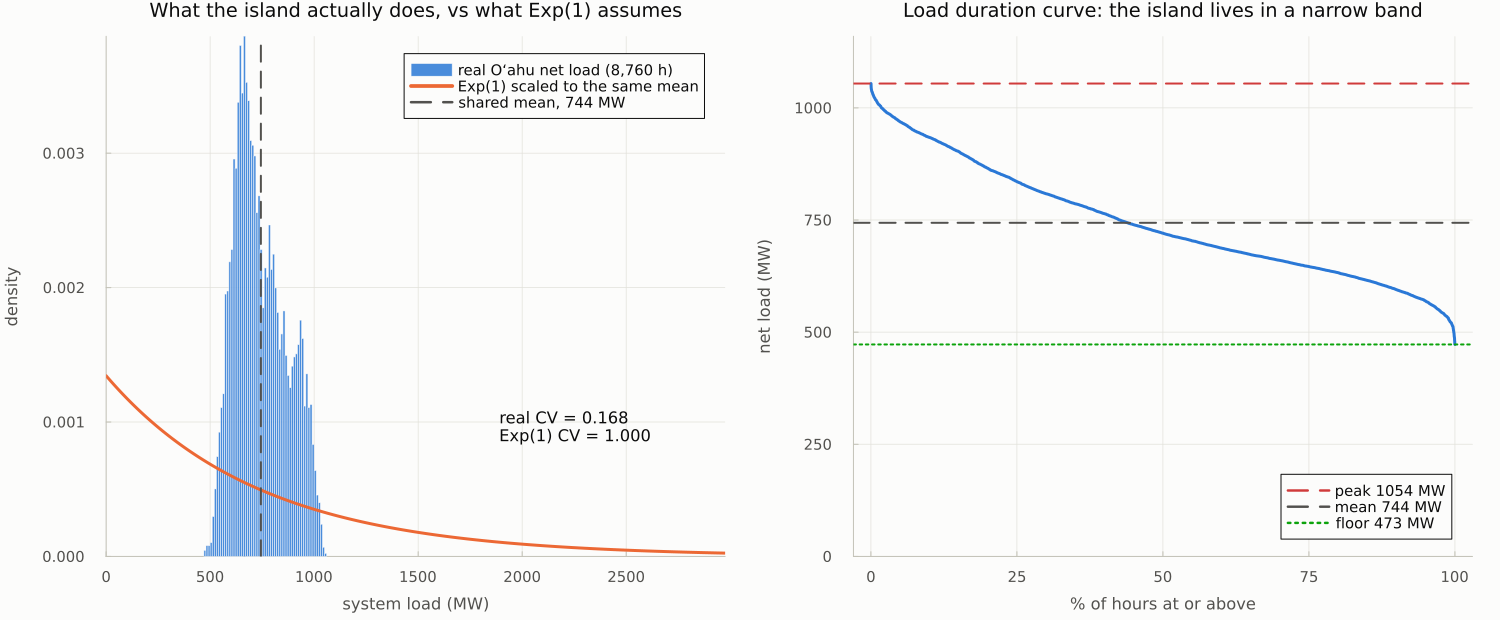
\includegraphics[width=\textwidth]{figures/q1_load_distribution.png}
\caption{Left: the empirical distribution of O\okina ahu net load against an
exponential density scaled to the same mean of \SI{743.9}{\mega\watt}; the
comparison is therefore purely one of shape. Right: the load duration curve. The
record occupies a band of roughly $0.64$ to $1.42$ times its own mean and never
leaves it.}
\label{fig:q1}
\end{figure}

\Cref{fig:merit} shows the fleet's merit order. Because real demand is confined to
a narrow band, it terminates in a narrow range of the cost stack: an average hour
is served to \SI{126.40}{\per\mega\watt\hour} and the annual peak only to
\SI{134.48}{\per\mega\watt\hour}, leaving the diesel peakers at
\SIrange{222}{238}{\per\mega\watt\hour} untouched.

\begin{figure}[t]
\centering
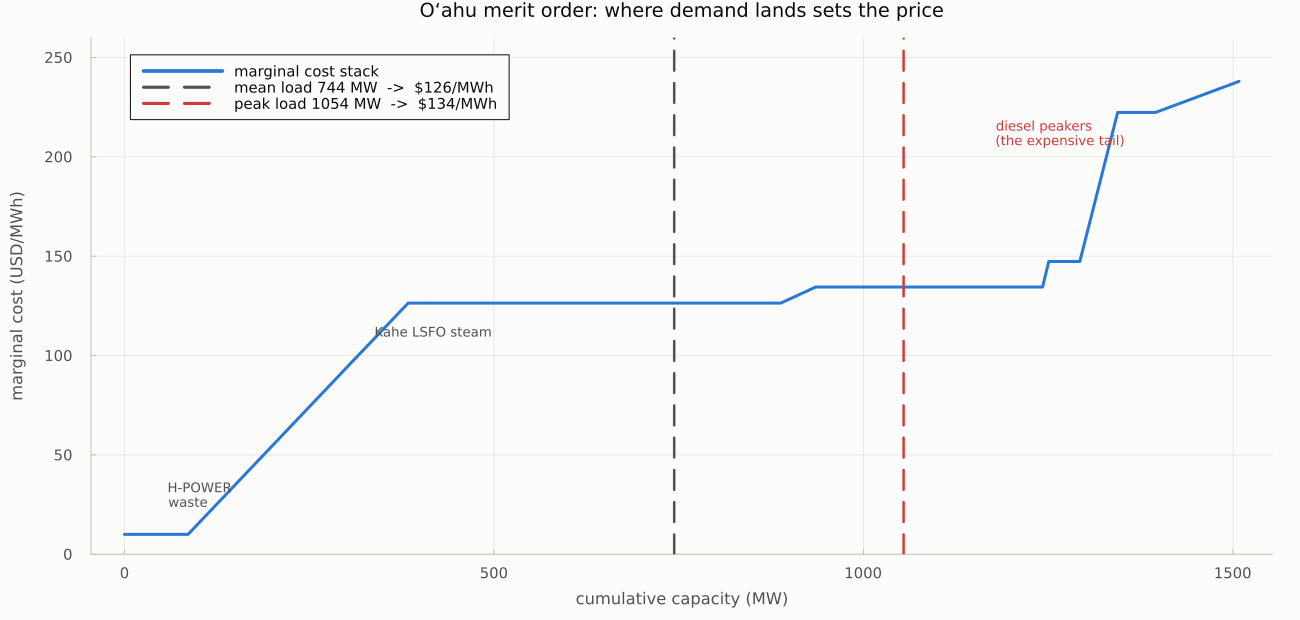
\includegraphics[width=0.92\textwidth]{figures/q1_merit_order.png}
\caption{O\okina ahu merit order. Cumulative capacity on the abscissa, marginal
cost on the ordinate. The step on which demand terminates is the system marginal
price.}
\label{fig:merit}
\end{figure}

\subsection{The IEEE 14-bus system and its calibration}

The IEEE 14-bus case is used as a controlled comparison. Two adaptations are
required. First, the published case lists no thermal ratings; since an
unconstrained network can never congest, ratings are assigned as
$\bar F_\ell = \max\{25,\; \lceil 1.5\,|F^{\text{base}}_\ell|\rceil\}$ from a
base-case solve. Second, and more importantly, the two systems must be placed
under comparable stress.

\begin{definition}[Utilisation]\label{def:util}
$\rho = M / \sum_g p^{\max}_g$, the ratio of design mean demand to nameplate
capacity.
\end{definition}

All three questions Q1--Q3 concern headroom, and headroom is governed by $\rho$.
Comparing a test system at its native $\rho = 0.335$ against an island at
$\rho = 0.493$ would compare calibrations rather than networks. We therefore set
the IEEE-14 mean to $\rho_{\text{O\okina ahu}} \times \SI{772.4}{\mega\watt} =
\SI{380.98}{\mega\watt}$, distributed across the eleven load buses in the
published proportions. The native case is retained as a reference point.

\begin{remark}[The linear cost simplification]\label{rem:linear-cost}
By \Cref{ass:standing}$(iii)$ we use only the linear cost coefficient, discarding
the quadratic term present in the IEEE-14 data. This keeps the program a linear
program with genuine locational marginal prices as duals, and matches the
convention used throughout the wider project. It has one consequence for Q1: under
linear costs the three units at buses 3, 6 and 8 share the maximum cost of
\SI{40}{\per\mega\watt\hour}, so ``the most expensive generator'' is properly a
most expensive \emph{tier}. Under the full quadratic cost the incremental costs at
full output would rank the units differently. We report the tier and label it as
such.
\end{remark}

% ==========================================================================
\section{Results: the IEEE 14-bus system}\label{sec:results14}
% ==========================================================================

\Cref{tab:q2} reports the three headline probabilities at $N = \num{10000}$,
with Wilson intervals.

\begin{table}[t]
\centering
\caption{IEEE 14-bus under Model A at $\rho = 0.493$, $N = \num{10000}$,
seed \num{20260908}. Intervals are Wilson score at $95\%$.}
\label{tab:q2}
\begin{tabular}{lcc}
\toprule
Event & Estimate & $95\%$ interval \\
\midrule
Costliest tier dispatched            & 59.63\% & $[58.66,\,60.59]$ \\
Load shedding required               & 41.58\% & $[40.62,\,42.55]$ \\
At least one branch at its limit     & 60.95\% & $[59.98,\,61.91]$ \\
\midrule
Mean branches at limit per replication & \multicolumn{2}{c}{$1.39$ of $20$} \\
Energy not served, share of demand drawn & \multicolumn{2}{c}{$8.29\%$} \\
Realised system $\CV$ & \multicolumn{2}{c}{$0.444$} \\
\bottomrule
\end{tabular}
\end{table}

The most informative comparison in \Cref{tab:q2} is between shedding frequency
and the frequency with which demand exceeds capacity. Demand exceeds
\emph{nameplate} capacity in only $\SI{2.87}{\percent}$ of replications, and
exceeds \emph{deliverable} capacity in $\SI{12.1}{\percent}$, yet shedding occurs
in $\SI{41.58}{\percent}$. Most adequacy failures on this network are therefore
failures of delivery, not of generation---consistent with
\Cref{cor:adequacy}, since a randomly oriented demand vector frequently has
$T^\star(\sigma)$ far below $T^\star(\bar\sigma)$.

\begin{figure}[t]
\centering
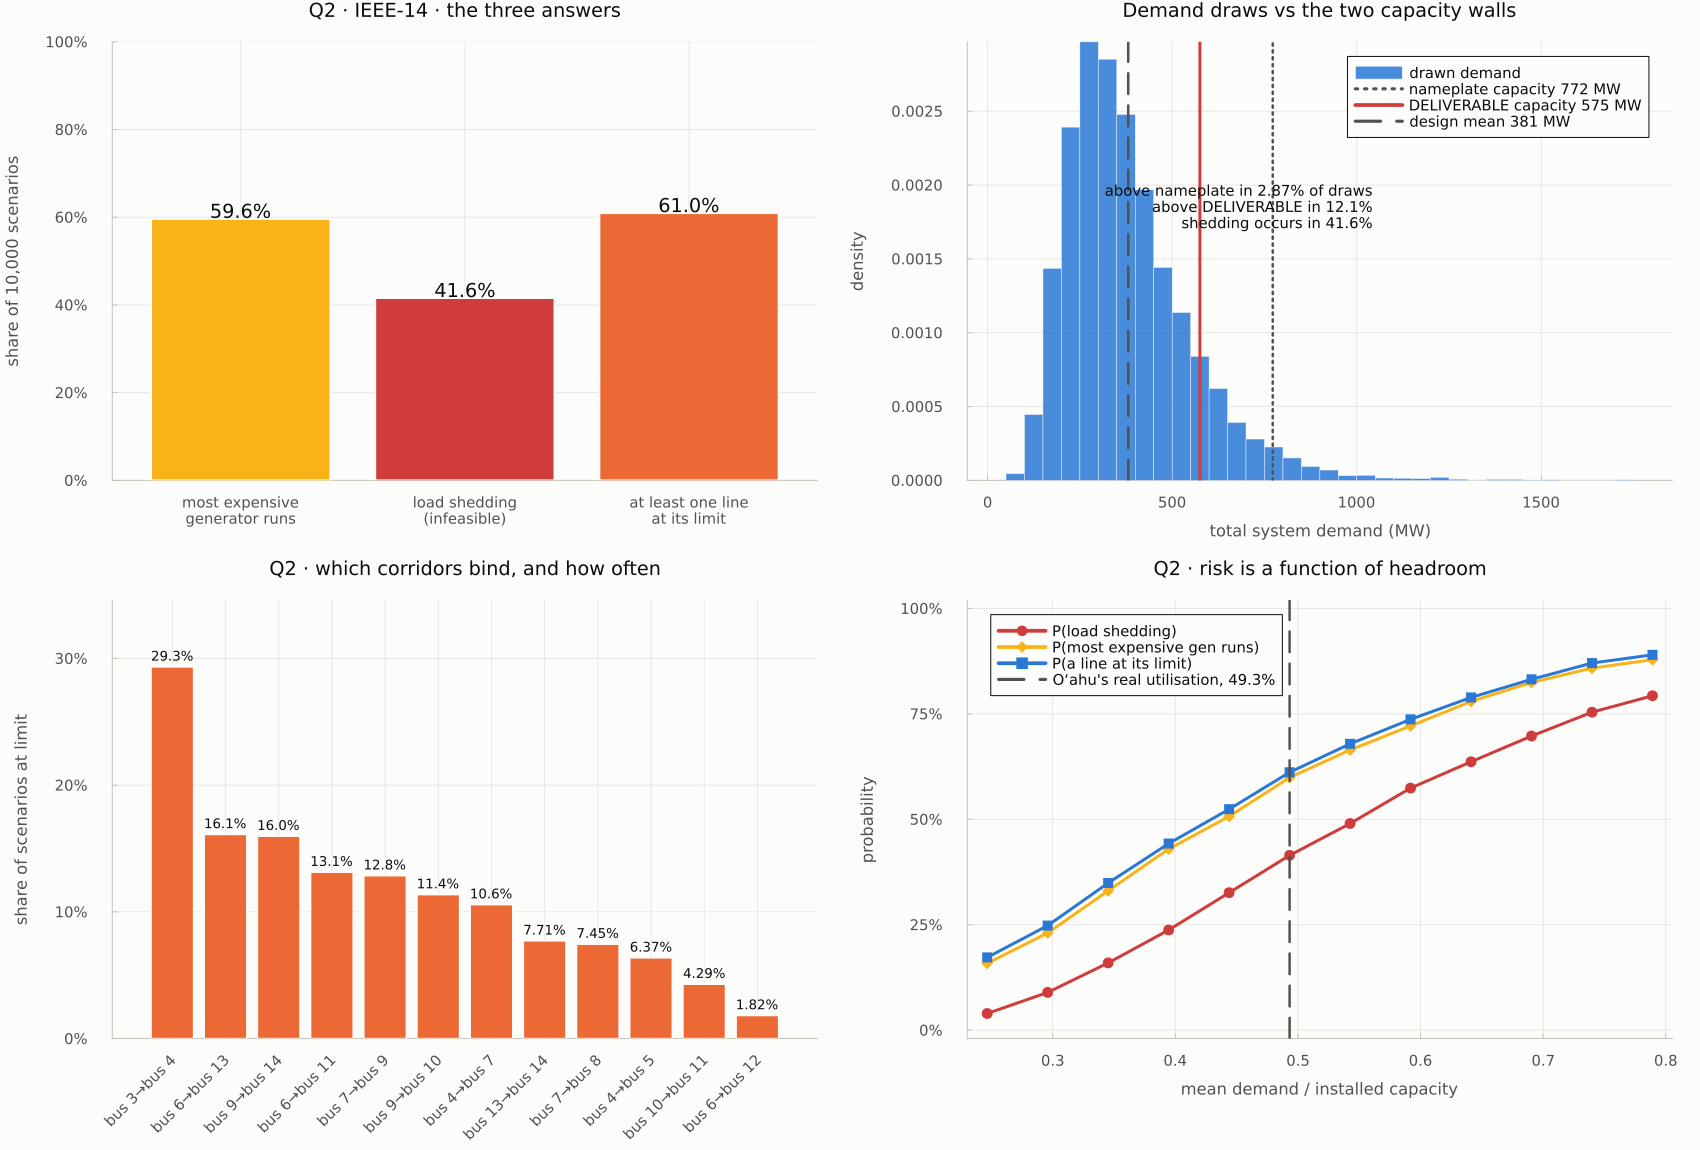
\includegraphics[width=\textwidth]{figures/q2_ieee14_dashboard.png}
\caption{IEEE 14-bus results. Top right: drawn demand against both capacity
walls. Bottom left: branch-level congestion frequency; the corridor from bus 3 to
bus 4 binds in $\SI{29.3}{\percent}$ of replications. Bottom right: the three
probabilities as functions of utilisation, with the network held fixed.}
\label{fig:q2}
\end{figure}

\paragraph{Sensitivity to utilisation.}
The lower-right panel of \Cref{fig:q2} sweeps $\rho$ from $0.25$ to $0.79$ with
the network---crucially including its thermal ratings---held fixed.
Shedding probability rises from $\SI{3.95}{\percent}$ to $\SI{79.30}{\percent}$
across that range. An earlier version of this sweep re-derived ratings at each
$\rho$ from the corresponding base case, which silently enlarged the network as
demand grew and produced a curve roughly four times too flat at the low end. We
record the error because it is easy to commit: a sweep over demand must not
re-tune the network.

\paragraph{Sensitivity to the random stream.}
Repeating the full experiment on four independent seeds gives shedding
probabilities $41.58$, $42.32$, $42.73$ and $\SI{43.10}{\percent}$---a spread of
$1.52$ points against a Wilson half-width of $0.97$, consistent with binomial
sampling error. The reported seed, fixed in advance as the presentation date,
sits at the low end of this range, so the headline figures are mildly
conservative.

% ==========================================================================
\section{Results: the O\okina ahu system}\label{sec:resultsoahu}
% ==========================================================================

\Cref{tab:q3} reports all three demand models on the unchanged O\okina ahu
network.

\begin{table}[t]
\centering
\caption{O\okina ahu, $N=\num{10000}$ per model, network identical throughout.}
\label{tab:q3}
\small
\setlength{\tabcolsep}{4.5pt}
\begin{tabular}{lccccc}
\toprule
Demand model & System $\CV$ & Costliest unit & Shedding & $\E[\text{shed}]$ & Branch at limit \\
\midrule
A\; independent $\mathrm{Exp}(1)$      & 0.532 & 5.48\% & 19.77\% & \SI{56.8}{\mega\watt} & 58.40\% \\
B\; common shock, $w=0.7$              & 0.708 & 5.20\% & 19.53\% & \SI{85.4}{\mega\watt} & 51.05\% \\
\rowcolor{gray!12}
C\; empirical resampling               & 0.168 & 0.00\% & \phantom{0}0.00\% & \SI{0.0}{\mega\watt} & 92.51\% \\
\bottomrule
\end{tabular}
\end{table}

Model B is instructive precisely because it moves so little. Introducing a common
island-wide shock leaves shedding \emph{frequency} essentially unchanged
($19.53$ against $\SI{19.77}{\percent}$) while raising expected unserved energy by
half (\SI{85.4}{} against \SI{56.8}{\mega\watt}). Correlation, on this network,
is a statement about the depth of failures rather than their incidence. As
\Cref{rem:w} notes, the comparison is not a clean isolation of correlation, since
$w$ also lowers nodal dispersion.

\begin{figure}[t]
\centering
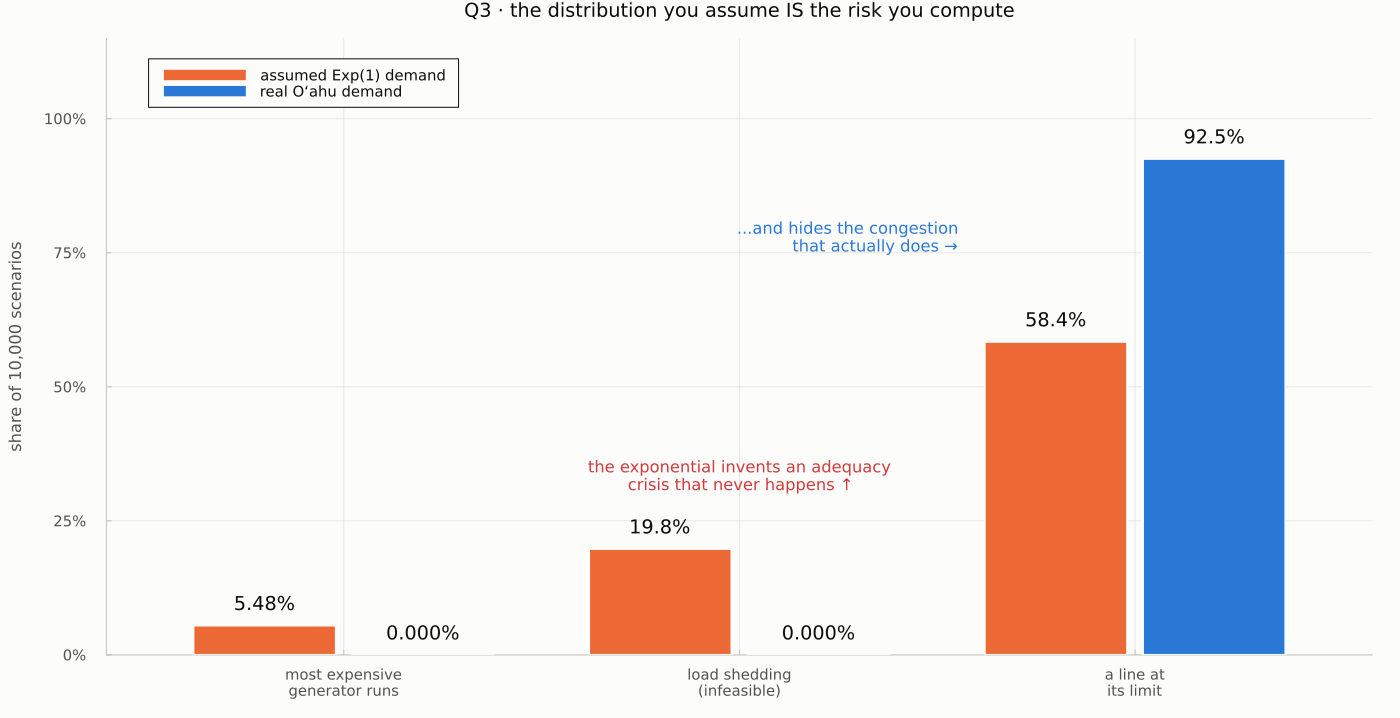
\includegraphics[width=0.95\textwidth]{figures/q3_headline.png}
\caption{The three questions answered under the assumed exponential demand and
under the empirical record, on an identical network.}
\label{fig:q3head}
\end{figure}

\paragraph{The binding corridor.}
Under Model C the branch from Ewa-West to Ewa-Central operates at a mean
$\SI{97.7}{\percent}$ of its \SI{400}{\mega\watt} rating and is at its limit in
$\SI{68.8}{\percent}$ of replications. Its structural role is visible from the
topology: the Kahe (\SI{582}{\mega\watt}) and Ewa-West (\SI{419}{\mega\watt})
generation sits behind it, and $\SI{84}{\percent}$ of island load sits in front of
it. This single branch is what reduces deliverable capacity to
\SI{1082.0}{\mega\watt} and, by \Cref{thm:modelC}, what sets the
$\SI{2.63}{\percent}$ adequacy margin.

\begin{figure}[t]
\centering
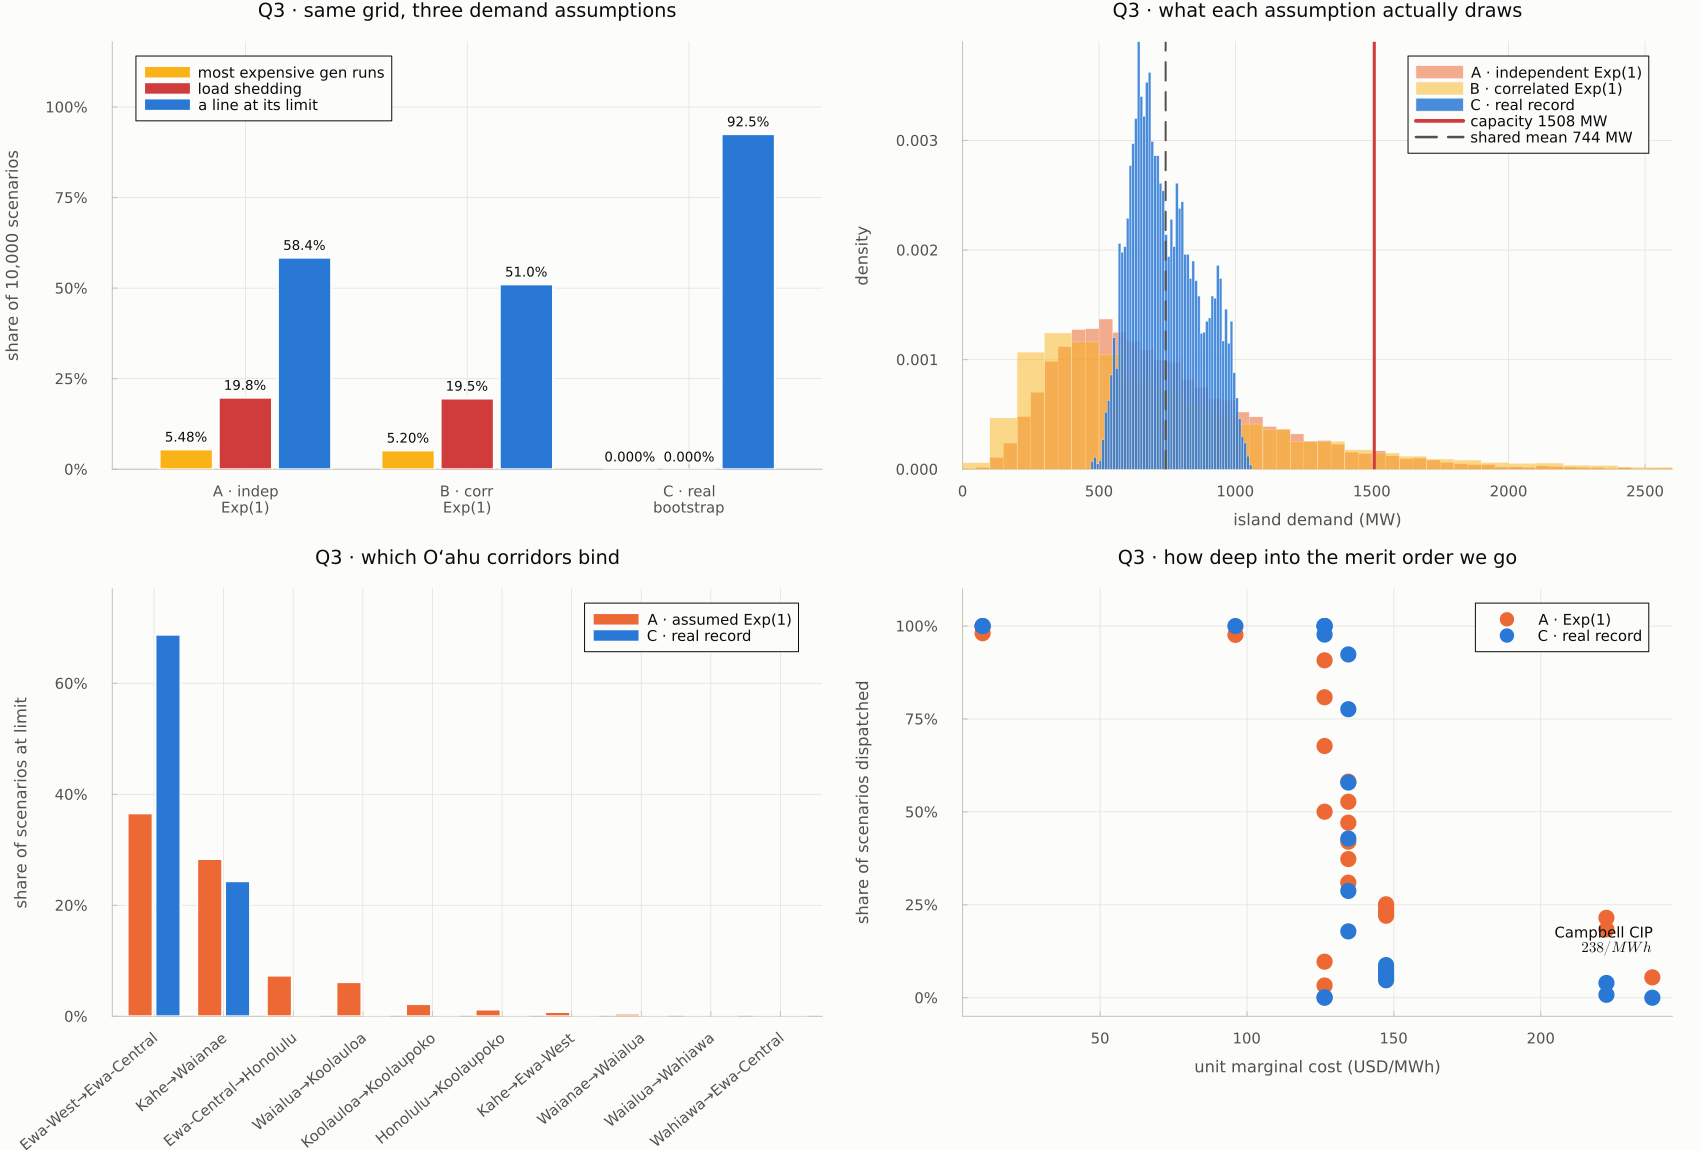
\includegraphics[width=\textwidth]{figures/q3_oahu_dashboard.png}
\caption{O\okina ahu under all three demand models: failure frequencies, the
demand distributions each model actually draws, branch-level congestion, and
depth of penetration into the merit order.}
\label{fig:q3dash}
\end{figure}

% ==========================================================================
\section{Misspecification: relocation rather than inflation}\label{sec:misspec}
% ==========================================================================

The comparison between rows A and C of \Cref{tab:q3} is the paper's empirical
centre. Holding the network, the solver, the estimator and the sample size fixed,
and changing only the demand distribution:

\begin{center}
\begin{tabular}{lccr}
\toprule
Quantity & Assumed $\mathrm{Exp}(1)$ & Empirical & Direction \\
\midrule
$\Prob(\text{shedding})$        & 19.77\% & \phantom{0}0.00\% & $\downarrow$ to zero \\
$\Prob(\text{costliest unit})$  & \phantom{0}5.48\% & \phantom{0}0.00\% & $\downarrow$ to zero \\
$\Prob(\text{branch at limit})$ & 58.40\% & 92.51\% & $\uparrow$ by $34$ points \\
\bottomrule
\end{tabular}
\end{center}

The two failure modes move in \emph{opposite directions}. This is the sense in
which the misspecification relocates risk rather than inflating it, and
\Cref{sec:geometry} supplies the mechanism for each half.

\paragraph{Why adequacy risk vanishes.}
By \Cref{cor:adequacy} shedding requires $T > T^\star(\sigma)$. Model A draws
directions with $T^\star(\sigma)$ frequently well below the design value
(\Cref{tab:tstar}: median \SI{1027.7}{\mega\watt}, first percentile
\SI{591.7}{\mega\watt}) and simultaneously draws magnitudes with a heavy right
tail, so the two cross often. Model C fixes the direction at a comparatively
favourable $\bar\sigma$ and caps the magnitude at the observed peak; by
\Cref{thm:modelC} the crossing never occurs.

\paragraph{Why congestion risk rises.}
By \Cref{prop:congestion-radial} congestion is approximately the event
$T > t_c$ with $t_c = \SI{585}{\mega\watt}$. The exponential places
$\SI{42.8}{\percent}$ of its mass below that threshold; the empirical record, which
never falls below \SI{472.6}{\mega\watt} and has a load factor of $0.706$, places
only $\SI{11.3}{\percent}$ there. Real load sits persistently in the band that
saturates the network, whereas the exponential repeatedly wanders out of it.

\paragraph{A general caution.}
The direction of misspecification bias is therefore mode-dependent, and cannot be
signed a priori from the tail weight of the assumed distribution. A heavier tail
increases the frequency of events defined by an upper threshold on a
\emph{radial} quantity (here, adequacy failure combined with the magnitude
crossing) but may either increase or decrease the frequency of events defined by
an \emph{interval} in that quantity. Congestion is of the second type: the
network is uncongested both when demand is small and---because an adequacy
failure is resolved by shedding at the constrained bus---the relationship at the
top of the range is not monotone either. Practitioners sometimes justify
fat-tailed demand models as ``conservative''. On the evidence here that
justification holds for adequacy and fails for congestion.

% ==========================================================================
\section{Limitations}\label{sec:limits}
% ==========================================================================

We list the limitations that bear directly on the conclusions.

\begin{enumerate}[label=\textbf{L\arabic*.},leftmargin=*,itemsep=0.35em]

\item \textbf{Model C fixes the demand direction.} By construction
$D = h_K s$, so all directional variation is suppressed. The zero shedding of
\Cref{thm:modelC} is thus a joint statement about the magnitude record \emph{and}
the population-share allocation, and \Cref{tab:tstar} shows the allocation is
comparatively favourable. A resampling scheme preserving the empirical spatial
copula would be the correct next step, and would likely produce a small but
nonzero shedding probability. The $\SI{2.63}{\percent}$ margin is the honest
headline, not the zero.

\item \textbf{Bus-level loads are proxied by population.} The allocation
$s$ is resident population share. Honolulu's commercial, hotel and military load
is not proportional to residence, so the true direction almost certainly differs
from $\bar\sigma$, and could be less favourable.

\item \textbf{The network is stylised.} Nine buses on a two-corridor
138\,kV ring with \SI{200}{\mega\watt} per circuit is a labelled technology
assumption, not the utility's model. The \emph{ranking} of corridors is a robust
finding; the exact percentages inherit the assumption. The Texas A\&M
\textsc{Hawaii40} synthetic case is the natural cross-check.

\item \textbf{No unit commitment.} \Cref{ass:standing}$(ii)$ sets
$p^{\min} = 0$. Real minimum stable output, start-up costs and minimum up/down
times would raise costs and could create adequacy failures at low demand that
this model cannot see.

\item \textbf{DC approximation and no contingencies.} Losses, reactive power and
voltage limits are absent, and the study is $N$-$0$. Given that the central
finding is a single binding corridor, an $N$-$1$ analysis is the most valuable
extension: the deliverable capacity of \Cref{tab:deliverable} would fall further
under credible outages.

\item \textbf{Congestion means saturation, not violation.} In a hard-constrained
formulation flows cannot exceed ratings; the constraint binds instead. Our
congestion statistic measures saturation. A companion unconstrained solve
measures how far over a rating flow would have gone, and is reported in the
repository.
\end{enumerate}

% ==========================================================================
\section{Conclusion}\label{sec:conclusion}
% ==========================================================================

Three conclusions survive the analysis.

First, the recourse formulation is the right instrument. Pricing unserved energy
at a value of lost load that exceeds the maximum nodal dual---not merely the
maximum generator cost, per \Cref{rem:voll}---makes the program feasible for
every realisation and converts adequacy failure into a measurable magnitude.

Second, the two failure modes have different geometry. Adequacy failure is
exactly the event $\lVert D\rVert_1 > T^\star(D/\lVert D\rVert_1)$
(\Cref{cor:adequacy}), a comparison against a direction-dependent threshold;
congestion is, on this network, approximately a fixed threshold on magnitude
alone (\Cref{prop:congestion-radial}). A demand model is therefore not adequate or
inadequate in general---it is adequate or inadequate \emph{for a given failure
mode}.

Third, the practical finding. Replacing an assumed $\mathrm{Exp}(1)$ demand with
\num{8760} hours of filed data eliminates an apparent $\SI{19.77}{\percent}$
shedding probability while raising congestion frequency by $34$ percentage
points. And the reserve margin that matters is not the
$\SI{43.0}{\percent}$ computed against nameplate capacity but the
$\SI{2.63}{\percent}$ computed against what the network can actually deliver---a
margin set by one \SI{400}{\mega\watt} corridor, behind which
\SI{426}{\mega\watt} of generation sits stranded.

\paragraph{Acknowledgements.}
This work was carried out as part of an ongoing research collaboration with
Adrian DeClerq, whose framing of the original question shaped the study.

% ==========================================================================
\appendix
\section{Data provenance}\label{app:data}
% ==========================================================================

\begin{table}[h]
\centering
\caption{Primary sources for the O\okina ahu model.}
\begin{tabular}{p{0.28\textwidth}p{0.62\textwidth}}
\toprule
Model element & Source \\
\midrule
Hourly load, \num{8760} obs.
& Hawaiian Electric, Final O\okina ahu Inputs Workbook~3, filed 2022-03-31;
2021 base scenario, reconstructed from underlying load, managed EV, distributed
PV, storage, efficiency and time-of-use layers. \\
Unit list, capacities
& U.S.\ EIA Form 860 (2024 final), summer capacity; operational Honolulu County
utility and contracted firm resources. \\
Heat rates
& U.S.\ EIA Form 923 (2024 final): electric fuel consumption divided by net
generation, at plant/prime-mover level. \\
Fuel prices
& Hawaiian Electric 2024 base forecast (LSFO, diesel, ULSD). \\
Buses and load allocation
& U.S.\ Census 2020 P.L.\ 94-171 county subdivisions via TIGERweb;
population-weighted tract centroids; loads allocated by resident population. \\
Topology
& Hawaiian Electric published \emph{Power Delivery} description: two-corridor
138\,kV ring; nine buses, ten branches, two independent loops. \\
Electrical parameters
& Technology defaults at 138\,kV, labelled as assumptions in the data files:
$0.8\,\Omega/\text{mile}$ reactance, \SI{200}{\mega\watt} per circuit. \\
IEEE 14-bus
& MATPOWER \texttt{case14}; ratings assigned per \Cref{sec:data}. \\
\bottomrule
\end{tabular}
\end{table}

% ==========================================================================
\section{Reproducibility}\label{app:repro}
% ==========================================================================

All results are produced by a Julia implementation using JuMP and the HiGHS
simplex solver. The random seed is \num{20260908} throughout. The computational
sequence is:

\begin{verbatim}
   julia "Q1 - hawaii data.jl"        # data audit, Figures 1-2
   julia "Q2 - ieee14 montecarlo.jl"  # Table 5, Figure 3
   julia "Q3 - oahu montecarlo.jl"    # Table 6, Figures 4-5
   julia anim_set8.jl                 # network animation
\end{verbatim}

The engine (\texttt{montecarlo.jl}) implements \Cref{def:program}, the three
demand models of \Cref{sec:demand}, the deliverable-capacity program
\eqref{eq:tstar}, and the Wilson interval \eqref{eq:wilson}. Case construction
for both networks is in \texttt{cases.jl}. Every figure and table in this paper
regenerates from those scripts; intermediate results are written to
\texttt{results/} as CSV.

\paragraph{Verification.} The formulation was checked against an independent
re-implementation of the power flow written from first principles. Over
\num{900} solved replications, energy balance closed to
$\num{6e-12}$\,MW, nodal Kirchhoff residuals recomputed from scratch to
$\num{1.2e-11}$\,MW, and the worst thermal-limit violation was
$\num{1.9e-12}$\,MW. The moment identities of \Cref{prop:cv,prop:mixture} were
confirmed against $\num{200000}$-draw simulations; the interval structure of
\Cref{prop:ray} was confirmed by fine scans along both design rays with no
violations; and \Cref{prop:voll} was checked on \num{6000} replications with no
counterexamples.

\end{document}
